\documentclass[12pt,a4paper,oneside]{report} 

\usepackage[utf8]{inputenc}
\usepackage[T1]{fontenc}
\usepackage[italian]{babel}
\usepackage{csquotes}

\usepackage[a4paper,margin=3cm]{geometry}
\usepackage{setspace}
\onehalfspacing  

\usepackage{lmodern}    
\usepackage{microtype}   

\usepackage[numbers,sort&compress]{natbib}

\usepackage{xcolor}
\usepackage[
    hidelinks,          
    colorlinks=true,
    linkcolor=black,
    citecolor=blue!50!black,
    urlcolor=blue!50!black
]{hyperref}

\usepackage{fancyhdr}
\pagestyle{fancy}
\fancyhf{} 
\fancyhead[LE,RO]{\thepage}
\fancyhead[LO]{\nouppercase{\rightmark}} 
\fancyhead[RE]{\nouppercase{\leftmark}}  
\setlength{\headheight}{14pt}

\usepackage{titlesec}
\titleformat{\chapter}[hang]
  {\bfseries\LARGE}
  {\thechapter\ \textcolor{gray}{|}}
  {0.6em}{}
\titlespacing*{\chapter}{0pt}{-6pt}{18pt}
\titleformat{\section}{\large\bfseries}{\thesection}{0.6em}{}
\titleformat{\subsection}{\normalsize\bfseries}{\thesubsection}{0.6em}{}

\usepackage{tocloft}
\setlength{\cftbeforechapskip}{6pt}
\setlength{\cftbeforesecskip}{2pt}

\usepackage{graphicx}
\usepackage{float}
\usepackage[labelfont=bf,font=small]{caption}

\usepackage{amsmath} 
\numberwithin{figure}{chapter}
\numberwithin{table}{chapter}

\usepackage[bottom]{footmisc} 
\setlength{\skip\footins}{12pt} 

\usepackage{listings}
\lstset{
    language=Python,
    basicstyle=\ttfamily\small,
    backgroundcolor=\color{gray!10},
    keywordstyle=\color{blue}\bfseries,
    commentstyle=\color{green!50!black}\itshape,
    stringstyle=\color{red!60!black},
    showstringspaces=false,
    breaklines=true,
    columns=fullflexible,
    frame=single,
    numbers=left,
    numberstyle=\tiny,
    numbersep=5pt
}

\usepackage{tikz}
\usetikzlibrary{positioning,shapes.geometric,arrows.meta}
\tikzset{
  mybox/.style={draw, rounded corners, fill=blue!10, align=center,
    minimum height=10mm, text width=6.2cm, inner sep=4pt},
  startstop/.style={draw, rounded corners, fill=red!15, align=center,
    minimum height=10mm, text width=6.2cm, inner sep=4pt},
  decision/.style={draw, diamond, aspect=2.2, fill=green!20, align=center, inner sep=1pt},
  arrow/.style={-{Stealth[length=2.4mm]}, thick}
}

\usepackage[section]{placeins}    
\usepackage{needspace}             
\usepackage{changepage}            

\usepackage{adjustbox}

\setcounter{topnumber}{2}
\setcounter{bottomnumber}{2}
\setcounter{totalnumber}{4}
\renewcommand{\topfraction}{.85}
\renewcommand{\bottomfraction}{.7}
\renewcommand{\textfraction}{.10}
\renewcommand{\floatpagefraction}{.80}

\setlength{\textfloatsep}{10pt plus 2pt minus 2pt}
\setlength{\floatsep}{8pt plus 2pt minus 2pt}

\captionsetup[table]{aboveskip=6pt, belowskip=4pt}
\captionsetup[figure]{aboveskip=6pt, belowskip=4pt}

\newenvironment{tabindent}[1][\parindent]{%
  \begin{table}[H]\begin{adjustwidth}{#1}{0pt}\centering}{%
  \end{adjustwidth}\end{table}}

\newenvironment{figindent}[1][\parindent]{%
  \begin{figure}[H]\begin{adjustwidth}{#1}{0pt}\centering}{%
  \end{adjustwidth}\end{figure}}

% --- (Opzionale) Glossario/acronimi ---
% \usepackage[acronym,toc]{glossaries}
% \makeglossaries

\setlength{\intextsep}{10pt}
\setlength{\textfloatsep}{12pt}
\captionsetup{width=.9\linewidth}

\title{doc}
\author{Valentina Piscopo}
\date{Agosto 2025}

\begin{document}

\maketitle

\begin{abstract}
      \noindent
      \textbf{Background:} Nel machine learning, l'effetto Rashomon descrive l'esistenza di molteplici modelli con prestazioni predittive equivalenti ma parametri diversi. Questo solleva una questione fondamentale per l'XAI: questi modelli forniscono spiegazioni simili per le stesse previsioni?

      \vspace{0.5em}

      \noindent
      \textbf{Metodi:} È stato costruito un Rashomon set di 10 reti neurali convolutional (CNN) con accuratezza entro l'1\% sul dataset MNIST. Per un campione di 10 immagini di test, sono state generate spiegazioni locali utilizzando tre metodi: Saliency, Integrated Gradients (IG) e LIME. Sono state quindi valutate la similarità tra le spiegazioni (tramite SSIM, correlazione di Pearson e Spearman, similarità del coseno e MAE) e la loro fedeltà (utilizzando le curve MoRF e la metrica AOPC).

      \vspace{0.5em}

      \noindent
      \textbf{Risultati:} La variabilità nelle spiegazioni è risultata essere principalmente guidata dalla scelta del metodo di XAI, non dal modello specifico all'interno del Rashomon set. La similarità inter-modello (stesso metodo, modelli diversi) è sistematicamente più alta della similarità intra-modello (metodi diversi, stesso modello). In termini di fedeltà, LIME ha ottenuto il punteggio AOPC più alto (0.7993), indicando che le feature che identifica sono le più decisive per la previsione del modello. Integrated Gradients ha mostrato un buon compromesso tra fedeltà (AOPC = 0.7511) e coerenza.

      \vspace{0.5em}

      \noindent
      \textbf{Conclusioni:} I risultati dimostrano che, in questo contesto, la scelta dell'algoritmo di spiegazione ha un impatto maggiore sulla spiegazione risultante rispetto alla variazione dei parametri del modello. Importante sottolineare l'importanza di valutare sia la similarità che la fedeltà per validare i metodi XAI, specialmente in scenari dove coesistono modelli equivalentemente accurati.
\end{abstract}
\newpage

\tableofcontents

\newpage

\maketitle

\chapter{Introduzione}

Quando ci affidiamo ai metodi di spiegazione per i modelli di \emph{machine
      learning}, sorge una domanda cruciale: \textit{quanto sono simili le
      spiegazioni prodotte da diversi algoritmi o modelli, e come possiamo misurare
      questa similarità?}

Nel contesto del \emph{Rashomon effect}
\cite{mueller2023rashomon,leventi2023consistency}, in cui coesistono molteplici
modelli con prestazioni equivalenti ma parametri differenti, questa domanda
assume un significato ancora più rilevante: se due modelli ottengono lo stesso
livello di accuratezza, possiamo aspettarci che spieghino le proprie decisioni
nello stesso modo?

Per affrontare questo problema, si adotta un approccio in tre fasi:
\begin{enumerate}
      \item Costruire un setup sperimentale con più modelli ugualmente accurati,
            appartenenti a un \emph{Rashomon set}, e analizzarli con diversi metodi di
            spiegazione.
      \item Applicare più metriche di similarità (ad esempio \emph{Structural Similarity
                  Index} — SSIM, correlazione di Pearson, similarità coseno, ecc.) alle
            spiegazioni prodotte.
      \item Confrontare i risultati per capire come varia la spiegazione in funzione sia
            del modello che del metodo scelto.
\end{enumerate}

Tuttavia, questo approccio presenta alcune criticità:
\begin{itemize}
      \item Due metodi di spiegazione, applicati allo stesso input, possono evidenziare
            regioni o feature completamente diverse come rilevanti.
      \item Metriche diverse possono portare a conclusioni contrastanti sul grado di
            similarità.
      \item L’assenza di un \emph{ground truth} della “spiegazione corretta” rende
            impossibile dichiarare in assoluto quale metodo sia “migliore”.
\end{itemize}

Per questo motivo, la sola similarità non è sufficiente a giudicare la qualità
di una spiegazione. È necessario integrarla con un’analisi della
\emph{fedeltà}, cioè della capacità della spiegazione di individuare feature
realmente decisive per la predizione del modello.

Un approccio comunemente adottato è l’analisi \emph{Most Relevant First} (MoRF)
\cite{samek2016evaluating}, in cui si mascherano progressivamente le feature
più importanti secondo la spiegazione e si osserva la velocità con cui decresce
la confidenza del modello. Ad esempio, in un classificatore di immagini, se
rimuovere la regione indicata come più rilevante provoca un crollo immediato
della probabilità predetta per la classe corretta, la spiegazione è considerata
fedele; al contrario, un impatto minimo sulla predizione indicherebbe una
spiegazione poco utile.

In letteratura non esiste una metrica unica e definitiva per la valutazione
delle spiegazioni \cite{adadi2018survey}, ma piuttosto un insieme di
prospettive complementari. Viene adottata quindi una doppia prospettiva:
\begin{itemize}
      \item analisi della \textbf{similarità} tra spiegazioni (intra-modello e
            inter-modello);
      \item analisi della \textbf{fedeltà} tramite MoRF e \emph{Area Over the Perturbation
                  Curve} (AOPC).
\end{itemize}

L’obiettivo finale è indagare se e come l’effetto Rashomon si manifesti non
solo nelle predizioni, ma anche nell’interpretabilità\footnote{In letteratura
      XAI, per interpretabilità si intende la possibilità di associare in modo
      comprensibile le decisioni di un modello alle caratteristiche rilevanti dei
      dati. Non va confusa con la sola \emph{fedeltà}, che riguarda invece quanto la
      spiegazione rifletta fedelmente il funzionamento interno del modello.},
valutando la coerenza e l’affidabilità dei metodi XAI in scenari controllati.

\chapter{Introduzione all’implementazione sperimentale}

L’esperimento è stato strutturato come una pipeline in più fasi, ciascuna con
un obiettivo specifico, seguendo approcci già consolidati in letteratura
\citep{mueller2023rashomon,leventi2023consistency,adadi2018survey}:

\begin{enumerate}
      \item \textbf{Costruzione di un Rashomon set}: una raccolta di modelli differenti,
            ma tutti con prestazioni simili sullo stesso compito di classificazione,
            in linea con la definizione proposta da \citet{fisher2019all}.
      \item \textbf{Applicazione di metodi di spiegazione}: generazione di spiegazioni locali
            per ciascun modello, su un insieme di dati di test, utilizzando diversi algoritmi XAI,
            tra cui Saliency \citep{simonyan2013deep}, Integrated Gradients \citep{sundararajan2017axiomatic}
            e LIME \citep{ribeiro2016lime}.
      \item \textbf{Valutazione della similarità delle spiegazioni}: confronto quantitativo
            tra le spiegazioni prodotte da modelli e metodi differenti, tramite varie metriche di similarità
            già impiegate in studi precedenti \citep{samek2016evaluating,adebayo2018sanity}.
      \item \textbf{Valutazione della fedeltà delle spiegazioni}: misurazione di quanto le
            feature individuate dalle spiegazioni siano realmente determinanti per le predizioni dei modelli,
            mediante tecniche come le curve \emph{MoRF} \citep{samek2016evaluating}.
\end{enumerate}

\begin{figure}[htbp]
      \centering
      \footnotesize
      \begin{tikzpicture}[
            node distance=10mm,
            box/.style={draw, rounded corners, fill=gray!10, align=center, minimum height=9mm, text width=8.8cm, inner sep=4pt},
            small/.style={draw, rounded corners, fill=gray!10, align=center, minimum height=9mm, text width=8.8cm, inner sep=4pt},
            arrow/.style={-{Stealth[length=2.4mm]}, thick},
            lbl/.style={circle, draw, fill=white, inner sep=1pt, font=\bfseries\scriptsize, yshift=6pt}
            ]

            \node (step1) [box] {Dataset MNIST \textit{(train/val/test)}};
            \node (step2) [box, below=of step1] {Addestramento di più CNN (stessa architettura)};
            \node (step3) [box, below=of step2] {Selezione del \textit{Rashomon set} \\ \small (modelli con accuratezza di validazione entro 1\% dal best)};
            \node (step4) [box, below=of step3] {Generazione delle spiegazioni \\ \small Saliency \;|\; Integrated Gradients \;|\; LIME};
            \node (step5) [box, below=of step4] {Valutazione della similarità \\ \small \emph{intra-modello} (tra metodi) \quad|\quad \emph{inter-modello} (stesso metodo) \\ \small Metriche: SSIM, Pearson, Spearman, Cosine, MAE};
            \node (step6) [box, below=of step5] {Valutazione della fedeltà \\ \small MoRF \& AOPC};
            \node (step7) [box, below=of step6] {Risultati \& interpretazione};

            \draw[arrow] (step1) -- (step2);
            \draw[arrow] (step2) -- (step3);
            \draw[arrow] (step3) -- (step4);
            \draw[arrow] (step4) -- (step5);
            \draw[arrow] (step5) -- (step6);
            \draw[arrow] (step6) -- (step7);

            % Etichette numerate
            \node[lbl] at (step1.north west) {1};
            \node[lbl] at (step2.north west) {2};
            \node[lbl] at (step3.north west) {3};
            \node[lbl] at (step4.north west) {4};
            \node[lbl] at (step5.north west) {5};
            \node[lbl] at (step6.north west) {6};
            \node[lbl] at (step7.north west) {7};

      \end{tikzpicture}
      \caption{Pipeline sperimentale ad alto livello: costruzione del \emph{Rashomon set}, generazione delle spiegazioni e valutazione di similarità e fedeltà.}
      \label{fig:pipeline_simplified}
\end{figure}

\section{Tecnologie}
Per implementare il workflow sperimentale descritto, è stato utilizzato un
ecosistema di strumenti largamente adottati in ambito \emph{explainable AI}, in
grado di garantire affidabilità, riproducibilità e scalabilità
\citep{adadi2018survey,mueller2023rashomon}:

\begin{itemize}
      \item \textbf{Python 3.x}: linguaggio di riferimento per la ricerca in XAI, scelto per la sua flessibilità e l’ampia disponibilità di librerie specializzate.
      \item \textbf{PyTorch}: libreria \emph{open-source} per il \emph{machine learning} e \emph{deep learning}, dotata di supporto nativo per l’autograd e adatta alla prototipazione rapida di modelli. Utilizzata per la definizione, l’addestramento e la validazione delle reti neurali, nonché per il calcolo dei gradienti richiesto dai metodi \emph{Saliency} e \emph{Integrated Gradients}.
      \item \textbf{Torchvision}: libreria complementare a PyTorch che offre dataset predefiniti (come MNIST), trasformazioni standard per immagini e modelli già pronti. Utilizzata per il download, la gestione e il preprocessing del dataset MNIST.
      \item \textbf{Captum} \citep{kokhlikyan2020captum}: libreria open source specifica per l’interpretabilità di modelli PyTorch. Fornisce implementazioni ottimizzate di numerosi metodi XAI, con API coerenti e facilmente integrabili. Utilizzata per generare le spiegazioni su tutti i modelli del Rashomon set, includendo metodi \emph{gradient-based} e \emph{model-agnostic} (\autoref{sec:gradient_vs_model}).
      \item \textbf{NumPy}: libreria fondamentale per il calcolo scientifico e la manipolazione efficiente di array numerici, usata per l’elaborazione dei dati, la normalizzazione delle spiegazioni e il calcolo di metriche.
      \item \textbf{Scikit-learn}: utilizzata per il calcolo di metriche (correlazioni, MAE) e per funzioni di utilità scientifica.
      \item \textbf{SciPy}: impiegata per calcolare correlazioni avanzate come Spearman e Pearson.
      \item \textbf{Scikit-image}: usata per il calcolo della metrica \emph{SSIM} (\emph{Structural Similarity Index}).
      \item \textbf{Matplotlib}: libreria di riferimento per la visualizzazione scientifica, utilizzata per produrre grafici e visualizzazioni qualitative delle spiegazioni.
      \item \textbf{Tqdm} \citep{tqdm}: per fornire barre di avanzamento e monitorare l’esecuzione di processi lunghi.
      \item \textbf{Glob, os}: per la gestione di file, directory e per il caricamento/salvataggio dei modelli, a supporto della riproducibilità.
\end{itemize}

\section{Riproducibilità e ambiente di sviluppo}
Per garantire la riproducibilità degli esperimenti e la gestione efficiente
delle dipendenze, sono state adottate le seguenti buone pratiche, in linea con
le raccomandazioni di \citet{pineau2020improving}:

\begin{itemize}
      \item \textbf{Gestione dell’ambiente con \emph{conda}}: tutte le dipendenze (librerie e relative versioni) sono state installate in un ambiente dedicato, così da poter replicare esattamente il contesto di esecuzione.
      \item \textbf{Controllo della casualità}: i \emph{random seed} sono stati fissati per NumPy, PyTorch e il generatore casuale di Python, così da rendere i risultati ripetibili anche in presenza di componenti stocastiche come l’inizializzazione dei pesi o lo \emph{shuffle} dei dati.
      \item \textbf{Salvataggio e caricamento dei modelli}: i modelli selezionati per il Rashomon set sono stati salvati su disco durante la fase di addestramento, evitando la ripetizione di processi costosi e permettendo il loro riutilizzo in fasi successive.
\end{itemize}

\section{Scelte implementative}
\label{sec:scelte_implementative}

Gli esperimenti sono stati condotti interamente su \textbf{CPU}, scelta che ha
avuto un impatto diretto sulle decisioni implementative. Lavorare senza GPU ha
imposto di trovare un equilibrio tra fedeltà delle spiegazioni e tempi di
calcolo ragionevoli, evitando configurazioni eccessivamente costose in termini
computazionali \citep{leventi2023consistency}.

\paragraph{LIME.}
Invece di operare a livello di singolo pixel (784 feature su MNIST), è stato
adottato un approccio \textit{patch-based}, suddividendo ogni immagine
$28\times28$ in blocchi $4\times4$ (\texttt{feature\_mask}), per un totale di
49 feature. Questa scelta è coerente con le raccomandazioni di
\citet{ribeiro2016lime} per ridurre il rumore e migliorare la stabilità:
\begin{enumerate}
      \item Riduce il rumore nelle spiegazioni: LIME soffre particolarmente quando le
            feature sono estremamente piccole, perché le perturbazioni casuali tendono a
            distruggere informazioni rilevanti.
      \item Riduce drasticamente il numero di perturbazioni necessarie per ottenere una
            regressione lineare stabile.
\end{enumerate}
Il numero di campioni $n\_samples$ è stato fissato a 200, per mitigare la variabilità intrinseca di LIME e migliorare la ripetibilità dei risultati.
Poiché ogni spiegazione richiede $n\_samples$ forward pass, è stato utilizzato \texttt{perturbations\_per\_eval=50} per elaborare perturbazioni in batch, riducendo così l’overhead di chiamate ripetute al modello.

\begin{figure}[htbp]
      \centering
      \setlength{\tabcolsep}{4pt}
      \begin{tabular}{cc}
            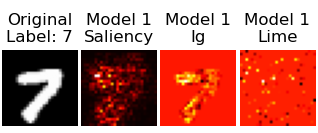
\includegraphics[width=0.45\textwidth]{images/lime_pixelwise.png} &
            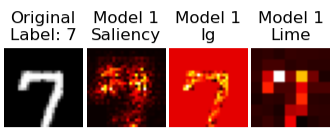
\includegraphics[width=0.45\textwidth]{images/lime_patch.png}                                                       \\
            \small (a) LIME pixel-wise (784 feature)                          & \small (b) LIME a patch 4$\times$4 (49 feature)
      \end{tabular}
      \caption{Confronto qualitativo delle mappe LIME prima/dopo il passaggio al masking a patch.
            L’approccio a patch riduce il rumore e mette a fuoco regioni più coerenti con la cifra.
            Immagini simili, stesso modello, $n_\mathrm{samples}=200$.}
      \label{fig:lime_before_after}
\end{figure}

\paragraph{Integrated Gradients (IG).}
È stato mantenuto il valore predefinito di \texttt{n\_steps} fornito da Captum.
Questo riduce il numero di forward pass necessari rispetto a valori più alti (che migliorano la precisione dell’integrazione ma aumentano i tempi di calcolo).
Come baseline è stata utilizzata un’immagine completamente nera (tutti zeri), scelta comune in letteratura per dataset con sfondo uniforme come MNIST \citep{sundararajan2017axiomatic}.

\paragraph{Saliency.}
Calcolata con il metodo base di Captum senza smoothing o normalizzazioni
aggiuntive, per preservare la semplicità e l’interpretabilità diretta delle
gradient map. Tecniche come SmoothGrad \citep{smilkov2017smoothgrad} avrebbero
aumentato la stabilità visiva, ma anche i tempi di calcolo di ordini di
grandezza.

\paragraph{MoRF/AOPC.}
La valutazione di fedeltà è stata implementata rimuovendo progressivamente le
feature più importanti in 10 step. La baseline di rimpiazzo è stata scelta come
\textit{media dell’immagine} anziché zeri, per minimizzare il rischio di
introdurre pattern artificiali fuori distribuzione che avrebbero potuto
alterare il comportamento del modello \citep{samek2016evaluating}.

\paragraph{Selezione del Rashomon set.}
La scelta dei modelli è stata guidata dalla \textit{validation accuracy},
selezionando tutti quelli entro l’1\% dal miglior modello, seguendo la
definizione operativa di \citet{mueller2023rashomon}. Questo garantisce che le
differenze osservate nelle spiegazioni non siano dovute a variazioni
significative in termini di performance di classificazione. Ogni modello è
stato salvato in formato \texttt{.pt} di PyTorch, assicurando la
riproducibilità esatta delle sperimentazioni.

\paragraph{Classe di riferimento per le attribuzioni.}
Le attribuzioni sono calcolate rispetto alla \textbf{classe vera} (\textit{true
      label}) e non a quella predetta. Questa scelta, già discussa in studi
precedenti \citep{arras2019evaluating}, mira a mantenere coerenza con il
\textit{ground truth}, evitando che errori di classificazione contaminino il
confronto tra spiegazioni. Tuttavia, si riconosce che questa impostazione non
riflette scenari reali, dove la classe vera potrebbe non essere disponibile —
rappresentando quindi una possibile minaccia alla validità esterna.

\section{Hyperparametri e setup sperimentale}

Nella Tabella~\ref{tab:hyperparams} sono riportati tutti i parametri e le
impostazioni utilizzate negli esperimenti, in modo da permettere la
riproducibilità dei risultati.

\begin{table}[H]
      \centering
      \renewcommand{\arraystretch}{1.2}
      \begin{tabular}{ll}
            \hline
            \textbf{Parametro}              & \textbf{Valore}                                             \\
            \hline
            Numero di modelli addestrati    & 10                                                          \\
            Epoche massime                  & 30                                                          \\
            Patience (early stopping)       & 3 epoche                                                    \\
            Soglia Rashomon                 & $1\%$ di differenza rispetto al miglior modello (val. acc.) \\
            Batch size                      & 64                                                          \\
            Baseline IG                     & immagine di zeri                                            \\
            Baseline MoRF                   & media dell’immagine                                         \\
            $n\_samples$ LIME               & 200                                                         \\
            Feature mask LIME               & blocchi 4×4 (49 feature totali)                             \\
            $n\_steps$ IG                   & valore predefinito Captum                                   \\
            Step MoRF                       & 10                                                          \\
            Classe di riferimento           & Classe vera (\textit{true label})                           \\
            Ottimizzatore                   & Adam                                                        \\
            Tasso di apprendimento iniziale & 0.001                                                       \\
            Dataset                         & MNIST (grayscale, 28×28)                                    \\
            \hline
      \end{tabular}
      \caption{Hyperparametri e setup utilizzati negli esperimenti.}
      \label{tab:hyperparams}
\end{table}

\chapter{Il Rashomon set}

Il \emph{Rashomon set} è una collezione di modelli diversi che ottengono
prestazioni simili su un determinato compito. Il termine deriva
dall’\emph{effetto Rashomon}, che descrive la possibilità che più spiegazioni,
tutte coerenti con i dati osservati, possano emergere per lo stesso fenomeno
\citep{mueller2023rashomon}. In ambito \emph{machine learning}, ciò implica
che, anche a parità di accuratezza, modelli con parametri differenti possono
fornire spiegazioni distinte per le proprie decisioni
\citep{fisher2019all,semenova2019existence}.

\section{Costruzione}
Il Rashomon set è stato costruito allenando più reti neurali della stessa
architettura (una CNN semplice) sul dataset MNIST. Ogni rete parte da una
diversa inizializzazione casuale dei pesi (\emph{random seed} differente) ed è
addestrata sugli stessi dati con un protocollo identico, che include la
suddivisione in training, validation e test set.

Durante l’addestramento è stata applicata la tecnica di \emph{early stopping}
\citep{prechelt1998early}: per ogni modello, l’allenamento viene interrotto se
le prestazioni sul validation set non migliorano per un numero prestabilito di
epoche consecutive. In questo modo si seleziona automaticamente la versione del
modello che ha ottenuto la miglior accuratezza sul validation, riducendo il
rischio di overfitting e garantendo un confronto equo tra i membri del set.

\section{Selezione}
Al termine dell’addestramento, sono stati selezionati tutti i modelli che
ottenevano un’accuratezza sul validation entro una certa soglia rispetto al
modello con la miglior performance. In questo esperimento la soglia è pari
all’1\%:

\[
      \mathrm{Accuracy}_{\mathrm{val}}(m) \geq \mathrm{Accuracy}_{\mathrm{val}}(m_{\mathrm{best}}) - \epsilon
\]
dove:
\begin{itemize}
      \item $\mathrm{Accuracy}_{\mathrm{val}}(m_{\mathrm{best}})$ è la miglior accuratezza sul validation ottenuta tra tutti i modelli addestrati;
      \item $\epsilon$ è la tolleranza fissata (0.01 in questo caso), in linea con la definizione operativa di Rashomon set \citep{fisher2019all}.
\end{itemize}

Questo criterio garantisce che i modelli selezionati siano equivalenti dal
punto di vista delle prestazioni predittive, pur potendo avere rappresentazioni
interne e logiche decisionali differenti
\citep{leventi2023consistency,mueller2023rashomon}.

\begin{lstlisting}[caption={Addestramento modelli e selezione Rashomon set}, label={lst:rashomon_training}]
for i in 1 to NUM_MODELS:
    imposta_seed(SEED + i)
    
    modello, acc_validazione = addestra_modello(dati_train, dati_val)
    
    if acc_validazione > best_acc_validazione:
        aggiorna_best_accuracy(acc_validazione)

    if acc_validazione >= best_acc_validazione - SOGLIA_RASHOMON:
        aggiungi_a_rashomon_set(modello)
        salva_modello(modello)
\end{lstlisting}

\section{Validazione dell’equivalenza (accuracies)}
\label{sec:rashomon_equivalenza}

Per verificare l’equivalenza operativa dei modelli selezionati (soglia 1\%
sulla validation), riportiamo le accuratezze di validazione e test per ciascun
modello e le statistiche riassuntive sull’insieme.

\begin{table}[H]
      \centering
      \begin{minipage}{0.90\linewidth}
            \centering
            \renewcommand{\arraystretch}{1.1}
            \setlength{\tabcolsep}{6pt}
            \begin{tabular}{rcc}
                  \hline
                  \textbf{Model} & \textbf{ValAcc} & \textbf{TestAcc} \\
                  \hline
                  9              & 99.08\%         & 99.03\%          \\
                  1              & 99.03\%         & 99.10\%          \\
                  8              & 99.03\%         & 99.02\%          \\
                  3              & 98.97\%         & 98.91\%          \\
                  4              & 98.95\%         & 99.04\%          \\
                  2              & 98.98\%         & 98.99\%          \\
                  7              & 98.89\%         & 98.86\%          \\
                  5              & 98.88\%         & 98.96\%          \\
                  0              & 98.83\%         & 99.01\%          \\
                  6              & 98.59\%         & 98.77\%          \\
                  \hline
            \end{tabular}
            \caption{Accuratezze per modello del Rashomon set (ordinate per ValAcc decrescente).}
            \label{tab:rashomon_acc_by_model}
      \end{minipage}
\end{table}

\begin{table}[H]
      \centering
      \begin{minipage}{0.70\linewidth}
            \centering
            \renewcommand{\arraystretch}{1.1}
            \begin{tabular}{lcc}
                  \hline
                          & \textbf{Media $\pm$ std} & \textbf{Min..Max}  \\
                  \hline
                  ValAcc  & 98.91\% $\pm$ 0.13\%     & 98.59\% .. 99.08\% \\
                  TestAcc & 98.97\% $\pm$ 0.09\%     & 98.77\% .. 99.10\% \\
                  \hline
            \end{tabular}
            \caption{Statistiche riassuntive sulle accuratezze del Rashomon set ($n=10$ modelli).}
            \label{tab:rashomon_acc_summary}
      \end{minipage}
\end{table}

\noindent
Le distribuzioni sono strette (dev.\,std $< 0.2$ p.p. su entrambi i set) e
i range rientrano nella soglia di selezione all’1\%, confermando l’\emph{equivalenza}
dei modelli ai fini delle analisi di similarità e fedeltà.

\section{Obiettivi}
La costruzione del Rashomon set serve a due scopi principali:
\begin{enumerate}
      \item \textbf{Studiare la variabilità delle spiegazioni}: se modelli ugualmente accurati forniscono spiegazioni simili, allora queste possono essere considerate robuste; se divergono, si manifesta l’effetto Rashomon anche nell’interpretabilità \citep{mueller2023rashomon}.
      \item \textbf{Testare i metodi di spiegazione}: usando un insieme di modelli equivalenti, è possibile valutare la coerenza e la fedeltà delle spiegazioni prodotte da diversi algoritmi XAI \citep{leventi2023consistency}.
\end{enumerate}

\section{Approfondimento}
\subsection{Equivalenza tra modelli}
Nel contesto di questo lavoro, due modelli sono considerati equivalenti se
soddisfano la condizione di soglia sull’accuratezza definita precedentemente.
Questa scelta è in linea con la definizione originaria di \emph{Rashomon set}
\citep{fisher2019all}, secondo cui l’insieme comprende modelli con prestazioni
quasi ottimali rispetto al miglior modello ottenuto. L’adozione di tale
criterio permette di:
\begin{itemize}
      \item Rispettare la formulazione teorica riportata in letteratura, in cui il Rashomon
            set è visto come una regione nello spazio dei modelli che contiene tutte le
            soluzioni con accuratezza comparabile \citep{mueller2023rashomon}.
      \item Esplorare la diversità interna tra modelli che, in termini predittivi, sembrano
            “uguali”, ma che possono differire nelle rappresentazioni interne e quindi
            nelle spiegazioni \citep{leventi2023consistency}.
\end{itemize}

\subsection{Perché utilizzare l’early stopping}
L’\emph{early stopping} \citep{prechelt1998early} è stato adottato per due
motivi principali:
\begin{itemize}
      \item \textbf{Evitare l’overfitting}: interrompendo l’addestramento quando le prestazioni di validazione smettono di migliorare, si evita che il modello memorizzi il training set perdendo capacità di generalizzazione.
      \item \textbf{Equità nel confronto}: applicando la stessa regola a tutti i modelli, ciascun membro del Rashomon set viene selezionato nelle condizioni di miglior equilibrio tra bias e varianza, come raccomandato nelle buone pratiche di confronto tra modelli \citep{goodfellow2016deep}.
\end{itemize}

Questo approccio assicura che la variabilità osservata nelle spiegazioni non
sia dovuta a un diverso grado di overfitting, ma a reali differenze nei
percorsi di apprendimento. Inoltre, fissando i \emph{random seed} per tutte le
componenti stocastiche (inizializzazione dei pesi, shuffle dei dati, generatori
casuali di librerie esterne) \citep{reimers2017reporting}, è possibile
distinguere la variabilità dovuta al caso da quella legata a differenze
strutturali nei modelli o nelle spiegazioni.

\subsection{Scelta dell’ottimizzatore: Adam.}
Per l’addestramento di tutte le reti neurali è stato utilizzato l’ottimizzatore
\emph{Adam} (\emph{Adaptive Moment Estimation}) \citep{kingma2014adam},
ampiamente adottato in ambito \emph{deep learning}. Adam adatta dinamicamente
il tasso di apprendimento per ciascun parametro in base alle stime dei momenti
del gradiente, permettendo:
\begin{itemize}
      \item Convergenza più rapida rispetto a metodi a tasso di apprendimento fisso.
      \item Maggiore stabilità anche in presenza di gradienti rumorosi, come avviene nei
            dati di immagini con variazioni locali.
      \item Ridotta necessità di un fine-tuning manuale del \emph{learning rate}.
\end{itemize}
L’uso di Adam ha reso possibile mantenere tempi di addestramento contenuti pur garantendo
una buona qualità della convergenza, aspetto particolarmente rilevante data
l’esecuzione esclusivamente su CPU.

\chapter{Metodi di spiegazione adottati}

Una volta selezionato il \emph{Rashomon set} dei modelli, il passo successivo
consiste nell’analizzare come ciascun modello giunge alle proprie decisioni.
Per questo scopo sono stati utilizzati tre metodi di spiegazione, scelti per
rappresentare sia approcci \emph{gradient-based} che \emph{model-agnostic}
\cite{adadi2018survey,guidotti2018survey}.

\section{Saliency}
Il metodo della \emph{saliency map} \cite{simonyan2013deep,samek2016evaluating}
è uno dei più semplici e diffusi. Calcola la derivata della probabilità (o
della logit) assegnata dal modello alla classe target rispetto a ciascun pixel
dell’immagine di input. I pixel associati ai valori assoluti più elevati sono
considerati più importanti per la decisione. Questo metodo è apprezzato per la
sua immediatezza, ma è noto per essere sensibile al rumore e
all’inizializzazione dei pesi del modello.

\section{Integrated Gradients (IG)}
Gli \emph{Integrated Gradients} \cite{sundararajan2017axiomatic} migliorano
l’approccio delle saliency map, correggendone alcune limitazioni. Calcolano il
contributo di ogni feature effettuando una media dei gradienti lungo un
percorso che va da una \emph{baseline} (nel nostro caso, immagine nulla) fino
all’immagine reale. Questo consente di ottenere spiegazioni più stabili e
coerenti, meno influenzate da piccole variazioni nei dati o nei parametri del
modello.

\section{LIME}
Il metodo \emph{LIME} (\emph{Local Interpretable Model-agnostic Explanations})
\cite{ribeiro2016lime} genera nuove istanze di input perturbate (ad esempio,
oscurando casualmente parti dell’immagine) e osserva come cambia la predizione
del modello. Successivamente, addestra un modello interpretabile locale (ad
esempio una regressione lineare) per stimare quali feature hanno avuto il
maggiore impatto sulla decisione del modello. Nel caso di MNIST, le
perturbazioni sono state effettuate non a livello di singolo pixel ma
aggregando in blocchi $4\times4$ per ridurre il rumore e i tempi di calcolo
(sezione~\ref{sec:scelte_implementative}).

\begin{lstlisting}[caption={Generazione delle spiegazioni}, label={lst:xai_generation}]
function genera_spiegazioni(modello, immagine, etichetta_vera):
    spiegazioni = {}
    
    spiegazioni["Saliency"] = calcola_saliency(modello, immagine, etichetta_vera)
    spiegazioni["IG"] = calcola_integrated_gradients(
        modello, immagine, etichetta_vera, baseline_zeri)
    spiegazioni["LIME"] = calcola_lime(
        modello, immagine, etichetta_vera,
        campioni=200, maschera_feature=FEATURE_MASK,
        baseline_media_pixel)
    
    return spiegazioni
\end{lstlisting}

\section{Motivazioni della scelta}
La combinazione di questi tre metodi consente di confrontare:
\begin{itemize}
      \item Approcci \emph{gradient-based} (Saliency, IG) e approcci \emph{model-agnostic}
            (LIME) \citep{simonyan2014deep,sundararajan2017axiomatic,ribeiro2016lime}.
      \item Metodi semplici e veloci con tecniche più robuste e computazionalmente costose.
      \item Stabilità delle spiegazioni e capacità di cogliere diversi aspetti
            dell’importanza delle feature \citep{samek2016evaluating,guidotti2018survey}.
\end{itemize}

\section{Gradient-based vs Model-agnostic} \label{sec:gradient_vs_model}
I metodi di spiegazione \emph{gradient-based} sfruttano direttamente la
struttura interna del modello: calcolano come varia la predizione rispetto a
piccole modifiche delle feature in input, utilizzando le derivate calcolate
tramite \emph{backpropagation}
\citep{simonyan2014deep,sundararajan2017axiomatic}. Questi metodi sono veloci
e, per modelli differenziabili come le reti neurali, forniscono indicazioni
precise sulle feature che guidano la decisione.

I metodi \emph{model-agnostic}, invece, trattano il modello come una “scatola
nera”: non richiedono accesso ai pesi o ai gradienti, ma solo la possibilità di
effettuare predizioni su input modificati
\citep{ribeiro2016lime,guidotti2018survey}. Questo li rende molto flessibili
(applicabili a qualsiasi modello), ma spesso più lenti e meno stabili, poiché
si basano su approssimazioni locali.

\chapter{Valutare la similarità tra spiegazioni}

Quando osserviamo due spiegazioni, possiamo essere tentati di giudicare
istintivamente se siano simili o meno. Ma le apparenze ingannano: differenze
visive possono non riflettere reali differenze nei pattern di importanza, e
viceversa. Nel contesto di un \emph{Rashomon set}, questa domanda diventa
cruciale: modelli diversi, ma ugualmente accurati, arrivano alle stesse
conclusioni per motivi simili, o per motivi profondamente diversi? Misurare la
similarità tra spiegazioni è un passo fondamentale per capire la robustezza e
la stabilità delle interpretazioni fornite dai metodi di \emph{eXplainable AI}
(XAI) \citep{samek2016evaluating, mueller2023rashomon}.

\section{Metriche adottate}
Per trasformare un concetto qualitativo come ``somiglianza visiva'' in numeri,
è necessario scegliere metriche che catturino aspetti diversi della relazione
tra due mappe di importanza:

\begin{itemize}
      \item \textbf{Structural Similarity Index (SSIM)} — valuta quanto due mappe siano simili in termini di struttura, considerando luminanza, contrasto e distribuzione spaziale. Un SSIM vicino a 1 indica che le due spiegazioni hanno pattern strutturali quasi identici \citep{wang2004ssim}.
      \item \textbf{Pearson correlation} — misura la correlazione lineare tra i valori di importanza, utile per capire se i valori crescono e decrescono insieme, indipendentemente dall’ordine dei pixel.
      \item \textbf{Spearman correlation} — analizza la correlazione tra i ranghi, quindi l’ordine relativo delle feature più importanti, anche se le scale numeriche sono diverse.
      \item \textbf{Cosine similarity} — confronta la direzione dei vettori di importanza, ignorando la loro lunghezza: due spiegazioni che mettono in evidenza le stesse zone avranno un valore vicino a 1, anche se una è ``più intensa'' dell’altra.
      \item \textbf{Mean Absolute Error (MAE)} — fornisce una misura diretta della differenza media assoluta nei valori di importanza; più è basso, più le mappe sono simili in valore assoluto.
\end{itemize}

La scelta di queste metriche consente di catturare diverse sfaccettature della
similarità: dalla struttura globale all’ordine delle feature, fino alla
corrispondenza numerica esatta \citep{leventi2023consistency,
      samek2016evaluating}.

\section{Procedura di confronto}
Il confronto è stato condotto calcolando le metriche per ogni immagine del test
set e per ogni coppia di spiegazioni, considerando due scenari distinti
\citep{bhatt2021evaluating, mueller2023rashomon, leventi2023consistency,
      krishna2022disagreement}:

\begin{enumerate}
      \item \textbf{Intra-modello} — confronto tra metodi diversi applicati allo stesso modello.
            In questo scenario si misura la coerenza tra approcci di spiegazione differenti:
            se producono mappe simili, significa che il modello è interpretato in modo coerente
            indipendentemente dal metodo XAI utilizzato.

      \item \textbf{Inter-modello} — confronto dello stesso metodo applicato a modelli diversi
            appartenenti al \emph{Rashomon set}.
            Qui si valuta la stabilità del metodo rispetto a variazioni nella struttura interna
            e nei parametri del modello, mantenendo invariato l’approccio di spiegazione.
\end{enumerate}

Le attribuzioni sono calcolate sempre rispetto alla \textbf{classe vera}
(\textit{true label})\footnote{La \emph{true label} è l’etichetta corretta
      associata a un singolo campione (es. la cifra “5” in un’immagine MNIST). Più in
      generale, il termine \emph{ground truth} indica il riferimento di verità
      utilizzato per valutare un modello, che nei problemi di classificazione
      coincide con le true labels.}. Questa scelta è stata adottata per garantire
coerenza con il \emph{ground truth} ed evitare che eventuali errori di
classificazione alterino il confronto. Tuttavia, essa rappresenta una
potenziale minaccia alla validità esterna: in scenari reali, la classe vera
potrebbe non essere disponibile e il comportamento del metodo rispetto alla
classe predetta potrebbe differire in modo significativo.

\section{Risultati quantitativi}
Le tabelle seguenti riassumono i valori medi delle metriche nei due scenari.

\FloatBarrier
\Needspace{18\baselineskip}

\begin{table}[H]
      \centering
      \renewcommand{\arraystretch}{1.05}
      \begin{adjustbox}{max width=\linewidth}
            \begin{tabular}{lccccc c}
                  \hline
                  \textbf{Coppia} & \textbf{SSIM}     & \textbf{Pearson}  & \textbf{Spearman} & \textbf{Cosine}   & \textbf{MAE}      & \textbf{n} \\
                  \hline
                  Saliency–IG     & 0.263 $\pm$ 0.064 & 0.529 $\pm$ 0.082 & 0.194 $\pm$ 0.052 & 0.651 $\pm$ 0.045 & 0.211 $\pm$ 0.059 & 100        \\
                  Saliency–LIME   & 0.178 $\pm$ 0.043 & 0.468 $\pm$ 0.063 & 0.392 $\pm$ 0.089 & 0.663 $\pm$ 0.037 & 0.177 $\pm$ 0.045 & 100        \\
                  IG–LIME         & 0.247 $\pm$ 0.054 & 0.421 $\pm$ 0.059 & 0.224 $\pm$ 0.059 & 0.780 $\pm$ 0.056 & 0.167 $\pm$ 0.046 & 100        \\
                  \hline
            \end{tabular}
      \end{adjustbox}
      \caption{Similarità \emph{intra-modello}: confronto tra metodi sullo stesso modello (media $\pm$ dev. std).}
      \label{tab:sim_intra}
\end{table}

\vspace{-0.3\baselineskip}

\begin{tabindent}
      \renewcommand{\arraystretch}{1.1}
      \begin{adjustbox}{max width=\linewidth}
            \begin{tabular}{lccccc c}
                  \hline
                  \textbf{Metodo} & \textbf{SSIM}     & \textbf{Pearson}  & \textbf{Spearman} & \textbf{Cosine}   & \textbf{MAE}      & \textbf{n} \\
                  \hline
                  Saliency        & 0.439 $\pm$ 0.067 & 0.612 $\pm$ 0.064 & 0.688 $\pm$ 0.062 & 0.727 $\pm$ 0.042 & 0.069 $\pm$ 0.012 & 450        \\
                  IG              & 0.711 $\pm$ 0.077 & 0.723 $\pm$ 0.079 & 0.516 $\pm$ 0.085 & 0.970 $\pm$ 0.013 & 0.083 $\pm$ 0.049 & 450        \\
                  LIME            & 0.639 $\pm$ 0.086 & 0.864 $\pm$ 0.051 & 0.541 $\pm$ 0.116 & 0.929 $\pm$ 0.028 & 0.093 $\pm$ 0.025 & 450        \\
                  \hline
            \end{tabular}
      \end{adjustbox}
      \caption{Similarità \emph{inter-modello}: stesso metodo su modelli diversi (media $\pm$ dev. std).}
      \label{tab:sim_inter}
\end{tabindent}

{\small \textit{Rimandiamo alla Sez.~\ref{sec:disc-tradeoff} per il trade-off tra stabilità e fedeltà.}}

\Needspace{8\baselineskip}

\begin{figindent}
      \centering
      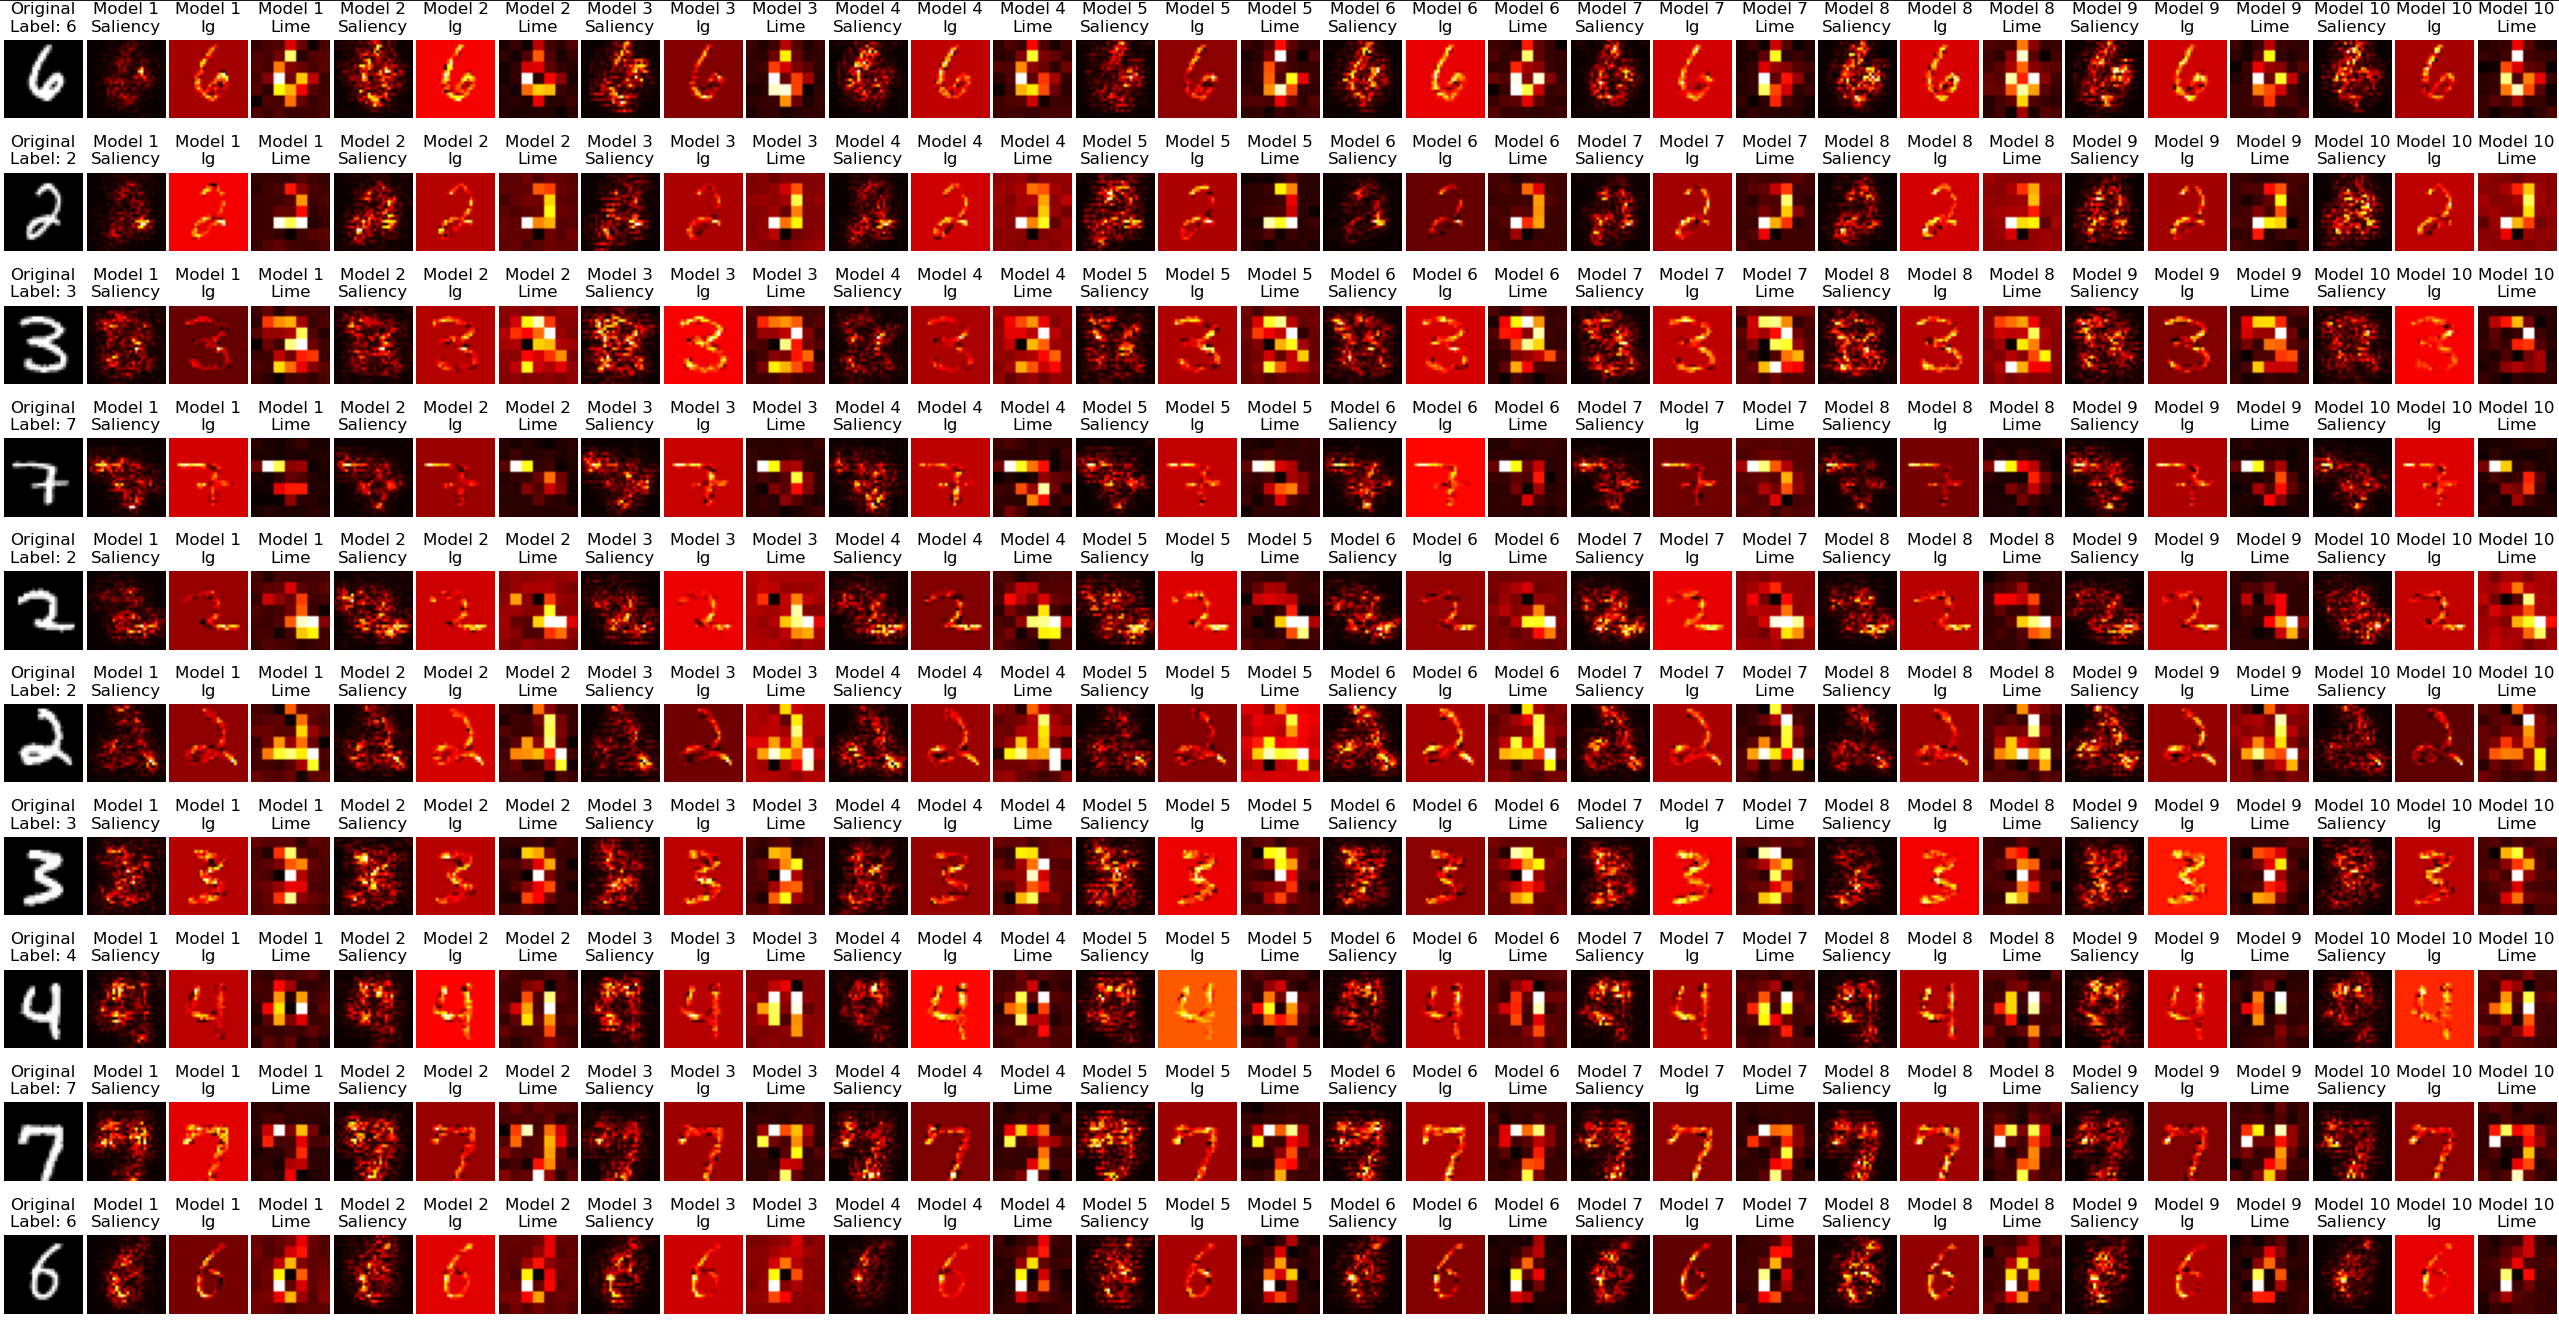
\includegraphics[width=\textwidth]{images/visualizzazione (2).png}
      \caption{Esempi di mappe di attribuzione per 10 modelli del Rashomon set su alcune immagini di test (MNIST).
            Ogni riga corrisponde a una diversa immagine originale, seguita dalle spiegazioni generate con Saliency, Integrated Gradients (IG) e LIME.
            Si osserva come le spiegazioni siano generalmente più coerenti \textbf{tra modelli} usando lo stesso metodo (colonne verticali),
            mentre differenze più marcate emergono \textbf{tra metodi} sullo stesso modello (blocchi orizzontali).}
      \label{fig:similarity_examples}
\end{figindent}

\subsection{Interpretazione}
I risultati mostrano una tendenza chiara e robusta:
\begin{itemize}
      \item La similarità \textbf{inter-modello} è sistematicamente più alta della
            \textbf{intra-modello} per tutte le metriche considerate. Questo indica che un
            singolo metodo tende a produrre spiegazioni coerenti anche al variare del
            modello del Rashomon set (es., SSIM: IG $0.711 \pm 0.077$, LIME $0.639 \pm
                  0.086$, Saliency $0.439 \pm 0.067$, $n=450$).
      \item La similarità \textbf{intra-modello} (metodi diversi sullo stesso modello) è
            sensibilmente più bassa, confermando che la scelta del metodo di spiegazione
            introduce le maggiori divergenze (es., SSIM: Saliency--IG $0.263 \pm 0.064$,
            Saliency--LIME $0.178 \pm 0.043$, IG--LIME $0.247 \pm 0.054$, $n=100$).
\end{itemize}

Guardando nel dettaglio, emerge un quadro coerente con la letteratura. In
\textbf{inter-modello}, \emph{Integrated Gradients (IG)} risulta il più stabile
in termini di direzione del vettore di attribuzioni (Cosine $0.970 \pm 0.013$),
mentre \emph{LIME} mostra la correlazione lineare media più alta (Pearson
$0.864 \pm 0.051$). \emph{Saliency} mantiene un buon ordinamento relativo delle
importanze al variare del modello (Spearman $0.688 \pm 0.062$). Le deviazioni
standard relativamente contenute in questo scenario confermano la coerenza tra
modelli dello stesso metodo.

In \textbf{intra-modello}, le similarità calano marcatamente: ad esempio,
\emph{SSIM} scende a $0.178$--$0.263$ con dispersioni non trascurabili ($\pm
      0.043$--$\pm 0.064$), e le correlazioni di rango (\emph{Spearman}) raramente
superano $0.392$ (Saliency--LIME $0.392 \pm 0.089$). Ciò suggerisce che metodi
diversi “raccontano storie diverse” anche quando osservano lo stesso modello:
differiscono nella \emph{forma} (SSIM), nell’\emph{ordinamento} (Spearman) e,
in parte, nell'\emph'{intensità/direzione} (MAE/Cosine) delle regioni ritenute
rilevanti.

In sintesi, nel contesto analizzato, la \textbf{scelta del metodo di
      spiegazione} ha un impatto più marcato sulla forma e sul contenuto della
spiegazione rispetto alla \textbf{scelta del modello}. Le deviazioni standard
riportate rendono esplicita questa variabilità: molto contenuta \emph{tra
      modelli} per uno stesso metodo (es., Cosine di IG $0.970 \pm 0.013$), più ampia
\emph{tra metodi} sullo stesso modello (es., Spearman $0.194 \pm 0.052$ fino a
$0.392 \pm 0.089$).

\chapter{Valutare la fedeltà delle spiegazioni: MoRF e AOPC}

Misurare la similarità tra spiegazioni è utile per capire se due metodi
``raccontano la stessa storia''. Ma una spiegazione può anche essere coerente e
stabile, eppure irrilevante per il modello. Per tale motivo serve valutare la
\emph{fedeltà}: le feature indicate come rilevanti sono davvero quelle che
guidano la decisione del modello?

\section{Procedura MoRF}
Il metodo \emph{Most Relevant First} (MoRF) è un approccio standard in
letteratura per testare la fedeltà delle mappe di importanza
\citep{samek2016evaluating,samek2017explainable}. L’idea è semplice: se le
feature indicate come importanti sono davvero decisive, rimuoverle dovrebbe
ridurre rapidamente la confidenza del modello nella classe target.

Il procedimento seguito è stato il seguente:
\begin{enumerate}
      \item Ordinare le feature o i pixel in base all’importanza decrescente indicata dalla
            mappa.
      \item Mascherare progressivamente le più importanti, in $K=10$ step uguali, partendo
            dalle più rilevanti.
      \item Usare come \emph{baseline} il valore medio dei pixel dell’immagine: questa
            scelta mantiene le immagini \emph{in-distribution}, evitando artefatti dovuti a
            valori estremi come tutto nero o tutto bianco.
      \item Dopo ogni mascheramento, registrare la probabilità che il modello assegna alla
            \textbf{classe vera} (\textit{true label}).
      \item Tracciare la curva MoRF, che mostra il decadimento della confidenza al crescere
            della porzione di immagine mascherata.
\end{enumerate}

\section{AOPC: Area Over the Perturbation Curve}
Per riassumere in un solo numero la qualità di una spiegazione, è stata
utilizzata la metrica \textbf{AOPC} (\emph{Area Over the Perturbation Curve}),
introdotta da \citet{samek2016evaluating}, calcolata come:

\[
      \mathrm{AOPC} = \frac{1}{K} \sum_{k=1}^K \left[ f(x) - f(x^{(k)}) \right]
\]

dove:
\begin{itemize}
      \item $f(x)$ è la predizione del modello sull’immagine originale.
      \item $f(x^{(k)})$ è la predizione dopo aver mascherato i primi $k$ blocchi di feature più importanti.
      \item $K=10$ è il numero di step di mascheramento.
\end{itemize}

Più il valore AOPC è alto, più la rimozione delle feature considerate
importanti provoca un crollo rapido della confidenza: un segno di elevata
fedeltà della spiegazione.

\begin{lstlisting}[caption={Procedura MoRF e calcolo AOPC}, label={lst:morf_aopc}]
function calcola_aopc(modello, immagine, mappa_spiegazione, steps=10):
    probas = []
    
    indici_importanti = ordina_pixel_per_rilevanza(mappa_spiegazione)
    
    for step in 0 to steps:
        immagine_modificata = maschera_pixel(immagine, indici_importanti, step)
        confidenza = predici_confidenza(modello, immagine_modificata)
        aggiungi(probas, confidenza)
    
    conf_iniziale = probas[0]
    differenze = [conf_iniziale - p for p in probas]
    aopc = media(differenze)
    
    return aopc, probas
\end{lstlisting}

\section{Risultati AOPC}
\begin{table}[h!]
      \centering
      \renewcommand{\arraystretch}{1.1}
      \begin{tabular}{lc}
            \hline
            \textbf{Metodo}      & \textbf{AOPC (media $\pm$ std)} \\
            \hline
            LIME                 & $0.7993 \pm 0.0948$             \\
            Integrated Gradients & $0.7511 \pm 0.1873$             \\
            Saliency             & $0.6568 \pm 0.1495$             \\
            \hline
      \end{tabular}
      \caption{AOPC per metodo (più alto = spiegazione più efficace), $n=100$.}
      \label{tab:aopc_results}
\end{table}

\begin{figure}[h!]
      \centering
      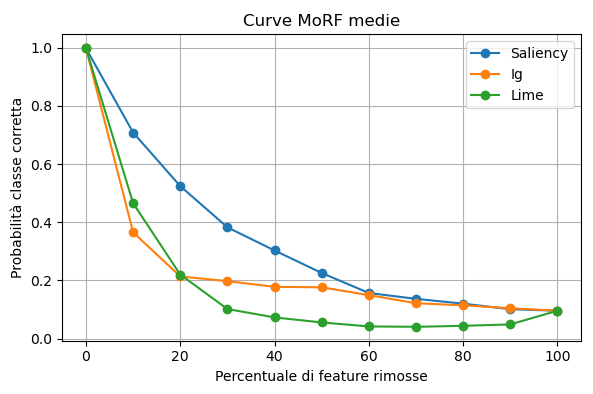
\includegraphics[width=0.75\textwidth]{images/grafMorf.png}
      \caption{Curve MoRF medie: andamento della probabilità della classe corretta al crescere della percentuale di feature rimosse.}
      \label{fig:morf_curves}
\end{figure}

\noindent
I risultati mostrano che:
\begin{itemize}
      \item \textbf{LIME} provoca il decadimento più rapido della confidenza media, segno che le feature evidenziate sono spesso effettivamente rilevanti per il modello.
      \item \textbf{Integrated Gradients} ottiene un valore intermedio, combinando buona fedeltà con alta coerenza inter-modello.
      \item \textbf{Saliency} registra valori più bassi, indicando che le feature evidenziate non sempre sono decisive per la classificazione.
\end{itemize}
{\small\textit{La relazione tra questi risultati e la stabilità inter-modello è discussa in
      Sez.~\ref{sec:disc-tradeoff}.}}

\noindent
Tali risultati vanno interpretati con cautela. LIME, pur essendo più rumoroso nelle visualizzazioni e meno coerente tra modelli, ottiene il punteggio AOPC più alto. Questo suggerisce che, quando individua una feature come rilevante, essa ha un impatto marcato sulla decisione del modello. \\
Integrated Gradients si colloca leggermente sotto, offrendo un equilibrio tra fedeltà elevata e coerenza inter-modello: un compromesso interessante in scenari dove entrambe le proprietà sono desiderabili. \\
Saliency, infine, mostra valori più bassi, segnalando che alcune feature evidenziate potrebbero non essere cruciali per la classificazione.

È importante notare che un AOPC elevato non implica necessariamente maggiore interpretabilità per l’utente umano: misura soltanto la capacità della spiegazione di individuare feature la cui rimozione comporta un rapido calo di confidenza del modello. Inoltre, i valori sono influenzati da scelte implementative come la baseline di mascheramento (media immagine) e, nel caso di LIME, dalla granularità delle perturbazioni (blocchi $4\times4$) e dal numero di campioni utilizzati.

\chapter{Discussione e implicazioni}

L’analisi ha mostrato che, nel contesto di un \emph{Rashomon set}, le
differenze tra metodi di spiegazione possono risultare più marcate di quelle
tra modelli ugualmente accurati. Questo rafforza l’idea che la scelta del
metodo XAI sia cruciale almeno quanto quella dell’architettura del modello,
quando l’obiettivo è comprendere le decisioni di un sistema di apprendimento
automatico.

\section{Trade-off tra fedeltà (AOPC) e stabilità (similarità)}
\label{sec:disc-tradeoff}

Mettendo in relazione i risultati di \emph{fedeltà} (AOPC;
Tab.~\ref{tab:aopc_results}) con quelli di \emph{stabilità} tra modelli
(similarità inter-modello; Tab.~\ref{tab:sim_inter}), emerge un chiaro
compromesso.

\paragraph{Evidenze quantitative.}
\textbf{LIME} massimizza in media la fedeltà (\emph{AOPC} $0.7993 \pm 0.0948$), indicando che le
regioni identificate come rilevanti causano un rapido decadimento della confidenza quando rimosse.
\textbf{Integrated Gradients (IG)} mostra invece una \textbf{stabilità inter-modello} molto elevata
(es. Cosine $0.970 \pm 0.013$, SSIM $0.711 \pm 0.077$), producendo mappe più coerenti al variare
dell’architettura. \textbf{Saliency} risulta intermedio/meno performante a seconda della metrica
(es. Spearman inter-modello $0.688 \pm 0.062$), suggerendo un buon mantenimento del \emph{ranking}
pur con minore fedeltà rispetto a LIME.

\paragraph{Quando privilegiare cosa.}
In contesti di \emph{debug/diagnosi}, dove è cruciale scoprire feature
realmente decisive, può essere preferibile \textbf{LIME} (maggiore AOPC),
accettando una variabilità superiore. In scenari di \emph{comunicazione verso
      utenti finali} o documentazione, dove la consistenza tra modelli è prioritaria,
risulta più adatto \textbf{Integrated Gradients} (maggiore stabilità).
\textbf{Saliency} può essere utile quando interessa soprattutto preservare
l’\emph{ordinamento relativo} delle importanze (correlazioni di rango), più che
la struttura spaziale o la magnitudine assoluta.

\paragraph{Limiti di interpretazione.}
Un AOPC elevato non implica automaticamente una migliore interpretabilità per
l’utente umano: misura l’impatto della rimozione di regioni ritenute
importanti, non la \emph{chiarezza} della spiegazione. Inoltre, le grandezze
osservate dipendono da scelte implementative come la baseline di mascheramento
per MoRF e la granularità/numero di campioni in LIME.

\section{Sintesi dei risultati principali}
\begin{itemize}
      \item La \textbf{variabilità intra-modello} è risultata più elevata della variabilità
            inter-modello, segnalando che metodi diversi possono produrre interpretazioni
            significativamente differenti anche sullo stesso modello.
      \item \textbf{LIME} ha mostrato la fedeltà più alta (AOPC), ma a costo di minore coerenza e maggiore rumorosità.
      \item \textbf{Integrated Gradients} ha offerto un buon compromesso tra stabilità e fedeltà, rendendolo adatto a scenari in cui entrambe le proprietà siano importanti.
      \item \textbf{Saliency} ha avuto prestazioni più basse in entrambe le metriche, suggerendo affidabilità limitata nel contesto MNIST e con configurazione base.
\end{itemize}

\section{Implicazioni pratiche}
I risultati suggeriscono che:
\begin{enumerate}
      \item La scelta del metodo XAI deve considerare sia la stabilità rispetto a
            variazioni del modello sia la fedeltà rispetto alla decisione effettiva, non
            solo la leggibilità visiva.
      \item In applicazioni critiche (es. medicina, finanza) può essere opportuno combinare
            più metodi per verificare la consistenza delle spiegazioni.
      \item Il \emph{Rashomon set} si rivela uno strumento efficace per validare la
            robustezza delle spiegazioni in scenari realistici, dove più modelli
            equivalenti possono coesistere.
\end{enumerate}

\section{Limiti e sviluppi futuri}
Le principali limitazioni riguardano:
\begin{itemize}
      \item l’uso di un dataset semplice (MNIST), che non riflette la complessità di domini
            reali;
      \item l’impiego di una sola architettura, che riduce la generalizzabilità dei
            risultati;
      \item l’analisi di un numero limitato di metodi XAI.
\end{itemize}

Lavori futuri potrebbero includere l’estensione a dataset più complessi (es.
CIFAR-10, ImageNet), il confronto tra architetture differenti, l’inclusione di
metodi più recenti (Grad-CAM, SHAP) e l’uso di metriche \emph{user-centered}
per valutare anche l’efficacia comunicativa delle spiegazioni.

\chapter*{Conclusioni}

Questo studio ha proposto un approccio sperimentale basato sul \emph{Rashomon
      set} per valutare la robustezza e la fedeltà delle spiegazioni fornite da
diversi metodi XAI. Il workflow ha previsto:
\begin{itemize}
      \item la costruzione di un insieme di modelli equivalenti in accuratezza;
      \item la generazione di spiegazioni tramite Saliency, Integrated Gradients e LIME;
      \item la valutazione della similarità (SSIM, Pearson, Spearman, Cosine, MAE) e della
            fedeltà (MoRF, AOPC).
\end{itemize}

L’analisi ha evidenziato che:
\begin{enumerate}
      \item la variabilità dovuta al metodo è maggiore di quella dovuta al modello;
      \item LIME eccelle in fedeltà ma presenta minore coerenza;
      \item Integrated Gradients bilancia stabilità e fedeltà;
      \item Saliency risulta meno performante in entrambi gli aspetti.
\end{enumerate}

In sintesi, la robustezza delle spiegazioni non può essere assunta a priori e
deve essere verificata sperimentalmente. L’approccio basato sul \emph{Rashomon
      set} fornisce un quadro metodologico utile e riproducibile per indagare tali
aspetti, ponendo le basi per futuri studi su dataset più complessi,
architetture eterogenee e metodi di spiegazione avanzati.

\clearpage
\bibliographystyle{plainnat} % coerente con natbib numeric compressed
\bibliography{references_base}

\end{document}
